\begin{figure*}[hbtp]
  \centering
  \subfigure{
    \label{fig:about-framework--all}
    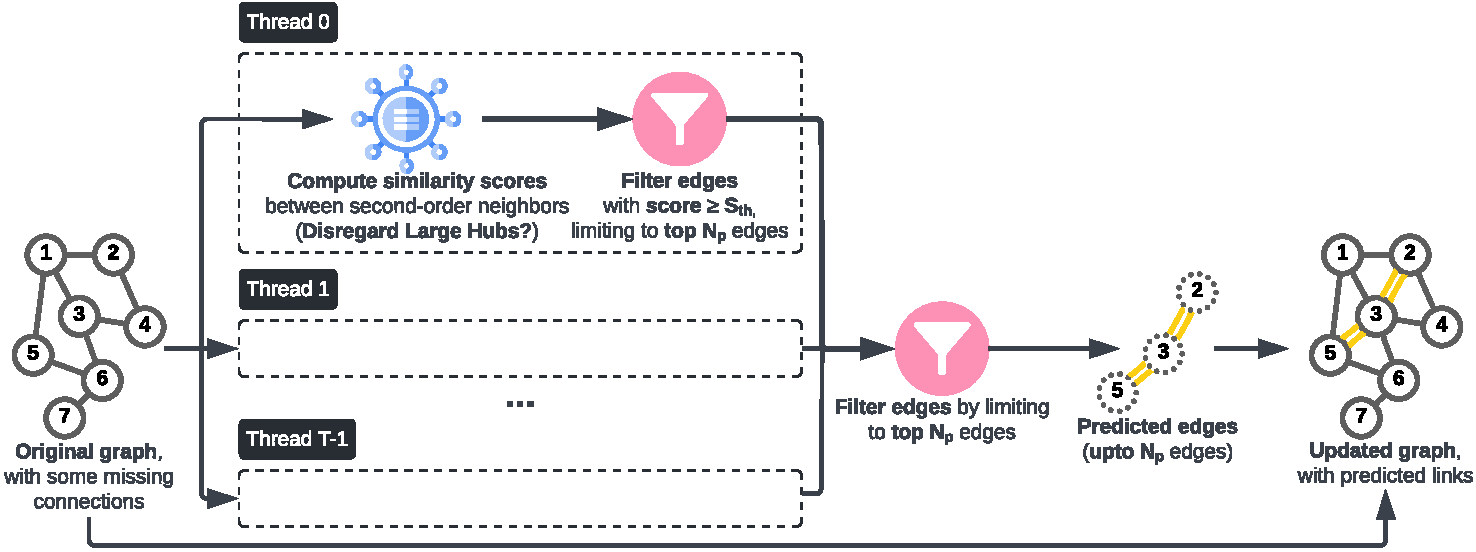
\includegraphics[width=0.98\linewidth]{out/about-framework.pdf}
  } \\[0ex]
  \caption{Framework diagram of our \textit{IBase} and \textit{DLH} approaches for link prediction. Here, $N_p$ denotes the maximum number of edges to predict, while $S_{th}$ indicates the threshold score for making a prediction.}
  \label{fig:about-framework}
\end{figure*}
% Framework diagram of our \textit{IBase} and \textit{DLH} approaches for link prediction. Given an original graph with some missing connections/edges, and $T$ threads, our parallel algorithms subdivide the vertices in the original graph into $T$ partitions (with dynamic scheduling), and compute similarity scores between non-connected second-order neighbors, from each source vertex, while optionally disregarding large hubs (DLH approach). The computed scores, along with their associated edges, are filtered to keep only the top $N_p$ edges with similarity score $\geq S_{th}$, independently by each thread. After this, the filtered edges and then merged together into a global list of edges, and filtered again to keep only the top $N_p$ edges --- finally obtaining the edges predicted by our approaches. The predicted edge can then be combined with the original graph to obtain an updated graph, which can then be used for running user-desired graph analytic upon.
